\scanpage{61}
\figure{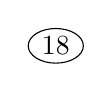
\begin{tikzpicture}\draw (0,0) ellipse (.35cm and .22cm);\node at (0,0) {\mspage{18}};\end{tikzpicture}}
avec $k$ successeur de $i$, il s'agit de singularité isolée, mais dans le cas de $V_{i,k}^k$ \unsure{général}, on peut trouver des singularités de type arbitraire bien sûr en fibre (prendre $X_i=X_i^*$ réduit à un pt !) — ce qui diminue l'intérêt, dans le cas de stratifications \unsure{tant soit peu} générales, des $V_{i,k}^j$ généraux comme ``pierres''. Les $V_{i,k}^{\unsure{j|i}}=V_{i,k}^*$ sont déjà plus intéressants, car \deleted{\unsure{ce sont}} c'est essentiellement un \inserted{germe d'} ouvert de $X_k^*$, donc non singulier — ce qui s'exprimera par le fait qu'on l'obtient comme un fibré sur $X_i^*$ non singulier, à fibre non singulière $V_{\unsure{z|Z},Z_{i,k}}^*$ \ldots

Donc nous allons dans la suite systématiquement essayer d'exprimer le maximum avec les $X_i^*$ et \inserted{les} $V_{ij}$, $V_{i,j}^*$ ``élémentaires'' ($j$ successeur de $i$), puis voir si certaines expressions peuvent prendre une forme plus sympathique en utilisant aussi \inserted{les $X_i^*$ et} les $V_{ij}$, $V_{i,j}^*$ avec $i\leq j$ sans plus — et dans un dernier temps seulement, peut-être (en égard au cas des diviseurs à croisements normaux) voir comment les $V_{i,k}^j$ s'insèrent dans ce formalisme.
\mspage{60}
